\textcolor{red}{
我们可以根据频谱数据识别出地海分界线,进而确定出岛屿在雷达坐标系中的位置,然后将其与地理坐标中的岛屿对应。因此,我们可以根据相同位置基准的偏差来获得PD变换系数。因此,这种方法最基础和最关键的部分是识别地海杂波识别。
}

一种改进方式是通过设置有源信标提供坐标配准修正参数,但是受到可部署区域的限制。由于陆地、海洋对雷达信号散射特性不同,可将陆地、海洋地理信息作为一类无源信标。通过区分识别地海杂波、构建地海边界轮廓、与先验地理轮廓信息匹配可同样提供坐标配准修正参数。传统地海杂波识别算法难以准确提取及表达地海杂波特征,从而在复杂电离层状况下地海杂波识别正确率较低。因此,如何发展一种更加准确的地海杂波类型识别方法,对天波超视距雷达电离层参数辨识及目标定位精度的提升有着重要意义。

为了提升目标定位经度,一种设想是利用检测区域内的有源/无源信标进行目标位置修正处理,通过对地海杂波特征深入分析和研究,分类识别出地海杂波,提取地海特征信息,并通过与地理位置匹配处理产生修正参数等,从而解决电离层模式配对等诸多工程应用问题,达到提升目标定位精度的目的。同时,在海杂波背景中探测海绵舰船目标的环境极其复杂,由于电波传播环境的影响(电离层时变和失真、易受干扰等),地海杂波附近存在很多虚警回波,严重影响目标的发现和自适应跟踪处理。,既能有效抑制虚警杂波,又能识别出感兴趣的低速舰船目标并稳定跟踪。

并对不同辐射源类别数、卷积神经网络层数、节点数、不同支持向量机参数与正确率进行了比较,讨论了相关参数对结果的影响。

对数据进行无监督或者半监督学习的方式进行训练。由于雷达信号量大,人为进行标记困难较大,本文计划进一步尝试无监督等减少人为标记的工作量。

另一方面,卷积减少了输出的空间范围,因此不可能使用卷积来重构具有相同空间范围的输入空间。
我们可以使用输入填充来解决这个问题。如果用零填充输入$x$,则第一卷积的结果可以具有比$x$更大的空间范围,因此第二卷积可以产生具有$x$的原始空间范围的体积。

因此,我们想要填充输入的零的数量是这样的:

\begin{equation}
	dim(x)=dim(decode(encode(x)))
\end{equation}

https://pgaleone.eu/neural-networks/2016/11/24/convolutional-autoencoders/

此处无监督聚类精度(unsupervised clustering accuracy, ACC)的定义为:
\begin{align}
	ACC &= \max\limits_m\frac{\sum_{i=1}^Ng(l_i,m(c_i))}{N} \\
	g(l_i,m(c_i)) &= \left\{
		\begin{array}{rcl}
		1       &      & l_i = m(c_i)\\
		0       &      & l_i \neq m(c_i)
		\end{array} \right. \nonumber
\end{align}
其中,$l_i$为真实的标签,$c_i$为算法的聚类结果,$m$是聚类结果与实际标签类别之间的一一对应,其遍历所有可能假设。
调整兰德指数(ARI)的定义为:
\begin{align}
	ARI &= \frac{RI - E[RI]}{max(RI)-E[RI]} \\
	RI &= \frac{a+b}{xxx}
\end{align}

\equref{equ:cae1}和\equref{equ:cae2}中的2D卷积操作由上下文决定。
一个$m\times m$矩阵和一个$n\times n$矩阵的卷积结果可能是$(m+n− 1) \times (m + n − 1)$(full convolution)也可能是$(m − n + 1) \times  (m − n + 1)$(valid convolution)。


% 我们在此通过对雷达信号序列的分析,利用深度学习方法对一维序列雷达信号进行处理。

% \equref{equ:loss_mse}利用均方误差函数作为损失函数。
% \begin{equation}
% C(w,b)\equiv \frac{1}{2n}\sum_x||y-a||^2
% \label{equ:loss_mse}
% \end{equation}
% 其中, $n$是训练输入数据的个数,$a$表示当输入为$x$时的输出向量。


% 这样就可以得到一种更简洁的表示法。这里激活函数 $ f(\cdot)$ 扩展为用向量(分量的形式)来表示,即$  f([z_1, z_2, z_3]) = [f(z_1), f(z_2), f(z_3)]$ ,那么,上面的等式可以更简洁地表示为:
% \begin{align}
% z^{(2)} &= W^{(1)} x + b^{(1)} \\
% a^{(2)} &= f(z^{(2)}) \\
% z^{(3)} &= W^{(2)} a^{(2)} + b^{(2)} \\
% h_{W,b}(x) &= a^{(3)} = f(z^{(3)})
% \end{align}

% 将上面的计算步骤叫作前向传播。用$  a^{(1)} = x$ 表示输入层的激活值,那么给定第$  l$ 层的激活值 $ a^{(l)}$ 后,第 $ l+1$ 层的激活值 $ a^{(l+1)}$ 就可以按照下面步骤计算得到:

% 将参数矩阵化,使用矩阵-向量运算方式,我们就可以利用线性代数的优势对神经网络进行快速求解。

% 要求解这样的神经网络,需要样本集  $ (x^{(i)}, y^{(i)})$ ,其中 $ y^{(i)} \in \Re^2$ 。

% 它同时,它可以通过池化(合并相邻特征)减少计算复杂度。
% 深度卷积神经网络与的两个主要区别是其

% ,这部分为需要进行主要设计,也是各种神经网络模型的主要区别之处。
% 为了增强其泛化能力,一般情况下有扩增路径(将多个分支包含在架构中)、金字塔形状(在整个架构中应该有一次整体的平滑的下采样,而且该下采样应该与信道数量的增长结合起来)、规范层输入(使层输入标准化,使所有输入样本更加平等)等各种设计法则,此部分需要根据实际问题以及测试结果不断调整。


% 首先介绍一种常用于工程实践中的地海杂波识别算法,单阈值法。通常,海洋和陆地杂波的差异在于,地杂波最大能量的频率几乎为零。然而,海杂波存在沿着零频率对称的有两个类似的峰,称为布拉格峰。因此,我们可以使用频率$ f $来判别频谱数据的地海杂波属性。
% \begin{equation}
% f_{i, j}= \mathop{\arg\max}_{f} \ \ x(i, j, f)
% \end{equation}
% $x(i, j, f)$ 是在频率 $f_{i, j}$下的能量值。在已知 $f_{i, j}$ 的情况下, 我们需要和阈值 $\eta$ 比较来判断其地海属性。
% \begin{equation}
% 	y_{i, j}= \left\{\begin{array}{ll}
% 		0&|f_{i, j}| > \eta, \\
% 		1&|f_{i, j}| < \eta
% 		\end{array}
% 		\right.
% \end{equation}
% 0代表海洋,1代表陆地。

在此基础上,我们使用相同的样本来分别训练和测试基于支持向量机的分类器和我们的算法。实验结果表明我们的算法具有更好的稳定性和准确性。

% \begin{figure}[H]
% 	\centering
% 	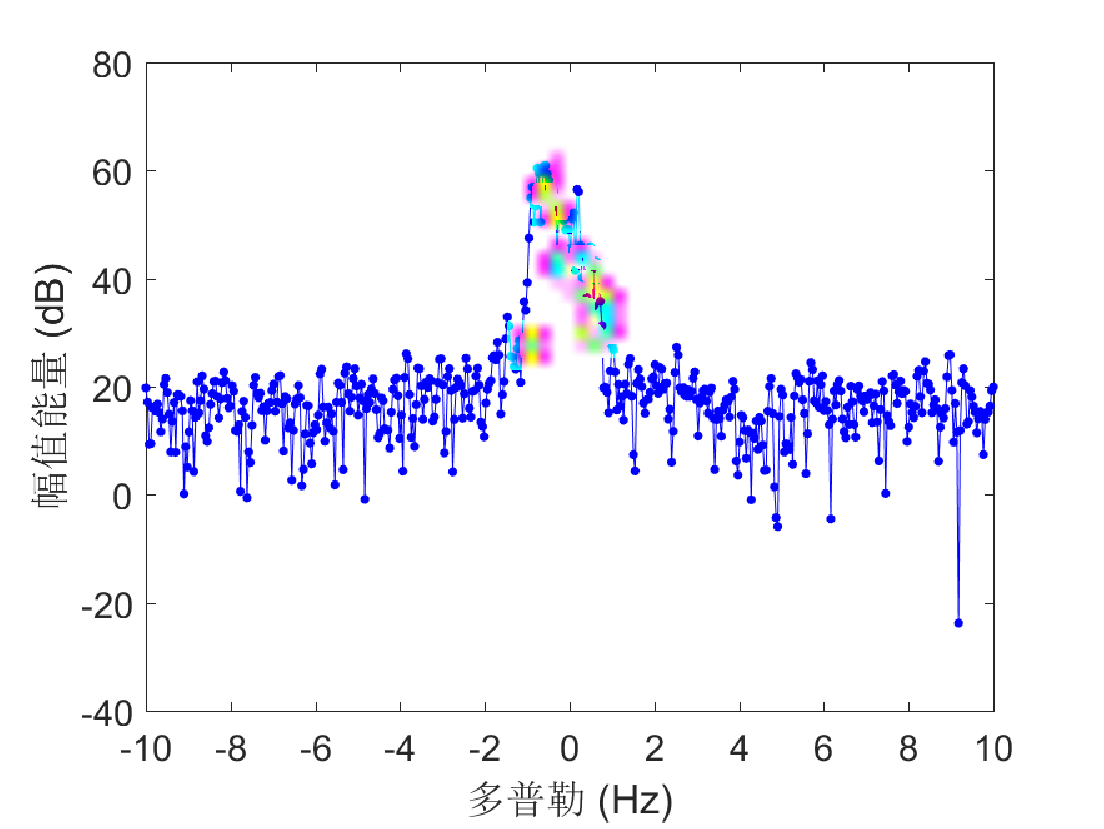
\includegraphics[width=6.67cm]{figures/othr/heatmap.pdf}
% 	\caption{某距离方位单元海杂波频谱数据关注度图。}
% 	\label{fig:visfeature1D}
% \end{figure}

% \textcolor{red}{
% 	识别结果的理论分析
% 	图\ref{fig:visfeature1D}中红色圆圈部分表示主要利用的特征所在多普勒频率,可以很直观地看出,对于图 xxx 这样的海杂波布拉格峰附近频点的数据被关注比较多,另一方面同时兼顾了其余频点的特征,提高了识别准确率。
% }
% 利用我们已经训练好的模型展示对于其最终判断测试结果为正或者为负主要利用的频谱特征点。


% 综上所述,我们这里的创新点有以下两个方面:第一个是我们提出了一种使用深度卷积神经网络方法利用频谱数据进行地海杂波分类的方法,克服了传统算法的挑战;另一方面,我们利用实际数据进行验证


% \subsection{增量学习}
% 随着时间的迁移,天波超视距雷达的观测范围或者是运行参数可能会发生大的变化,使得目前的训练结果无法很好的满足新的需求,于是本文设计了一种基于增量学习的训练方法。对于新的频谱数据集一般会相比于原数据集更小,所以重新训练常常无法取得一个很好的结果,对原始训练结果进行微调是十分必须的。一般来说,DCNN的比较靠前的层所包含的特征更一般化,而更靠后的层会越来越特定于该频谱数据中包含的分类细节。所以一个比较好的方案是保持前面的一些层固定,只微调网络后面的一些层。另一方面,由于原始数据训练出的DCNN的权重是相对较好的,故需要给正在被微调的DCNN权重使用较小的学习率和学习衰减率。


% \textcolor{red}{;对雷达有意调制和无意调制这两种脉内调制形式进行建模,综合分析其对应的各种特征(瞬时自相关、相位差分法、模糊函数等建立基于深度学习的分类结构;结合大量数据,对结构进行验证和调整;基于实际数据,对算法的各种特性进行验证。}

% 从中选取三个类别的I/Q信号图,得到如图 \ref{fig:IQs} 所示,从中可以看出各个信号之间的差距并不明显,因此我们对原始信号进行了优化。

% 从上面的分析可以看出,核参数影响着映射函数、进而影响样本子空间的复杂度。最后会影响分类器性能的好坏。惩罚参数作用是在数据子空间中调节支持向量机置信区间的范围。这些都说明了惩罚参数和核参数的选择非常重要。

% 对于本章这个Open Set 识别问题,我们需要用别的参数衡量识别的准确度。利用文\cite{scheirer2013toward}中提出的通过训练类别的个数和测试类别的个数来描述数据集的开放度(openness),如\equref{equ:openness}所示
% \begin{equation}
% 	openness = 1-\sqrt{\frac{2t}{\eta m+e}}
% 	\label{equ:openness}
% \end{equation}
% 其中,$t$表示训练类别的个数, $\eta $表示目标类别的个数,$m$ 表示分类器输出类别的个数,对于本章的识别问题,有$\eta=1$,$e$表示验证类别的个数,有$e>t,e>\eta$。对于一个完全的闭集识别问题有$e=t$意味着未知类别数据集为空。

% 另一方面,用F-measure 来衡量该分类器对于未知分类样本的处理情况。其定义为:
% \begin{equation}
% 	\text{F-measure}=2\times\frac{p\cdot r}{p+r}
% \end{equation}
% 其中,$p$表示精确率(precision),$p=\frac{TP}{TP+FP}$,其中$TP$表示正类识别为正类的样本数目,$FP$表示负类识别为正类的样本数目。$r$表示召回率(recall),$r=\frac{TP}{TP+FN}$,其中$FN$表示正类识别为负类的样本数目。

% openness 与 F-measure 曲线图


目前的研究重点主要集中在不同调制类型的辐射源的识别方面,而关于参数不同或者参数相近乃至相同的辐射源识别的研究较少,限制了其实际应用。


随着科学技术的进步,现代战场形势瞬息万变,信息对抗在现代军事中的作用越来越重要。纵观整个20世纪所爆发的两次世界大战和数次局部战争、21世纪初的美阿、美伊之战以及2017年闹得沸沸扬扬的韩国的萨德事件,无一不昭示着现代战争在很大程度上是信息战。
信息战的一个重要特征是利用各种探测、感知手段,借助计算机网络、通信技术,对敌人的作战部队以及地理信息等情况做到精确的探测评估,这样才能做到“知己知彼,百战不殆”。在信息化战争中,对于空间信息探测、敌方势力的识别、跟踪、定位等功能,主要依靠电子技术来完成\ucite{顾耀平2006电子战发展趋势分析, 孙德海2003国外电子战发展综述及对我国电子战研究的思考, 炜森1996综合电子战新技术新方法, 孙纪尧2014电子战}。

\item 根据雷达信号特征,对本文算法进一步调整。在天波雷达地海杂波识别中,我们现在把已有数据分成几组,分别进行训练。我们计划尝试使用一些方法对这些数据进行融合分析,以获得一个可以适应各种数据情况的模型。对于辐射源识别,利用更多的数据对算法进行进一步的验证,目前类别较少的情况下,部分结果会对选择的类别具有一定的依赖性,另一方面是选取更多更合适的特征进行训练学习。



\subsection{无监督聚类算法研究现状}
由于有监督学习需要对大量的数据进行打标签,这个过程通常需要花费大量的时间与精力。无监督学习也即聚类算法,克服了此问题,因此国内外学者对各个领域的聚类算法进行了广泛研究,产生了各种不同类型的聚类算法,例如层次聚类\ucite{heller2005bayesian},基于质心的聚类方法\ucite{lloyd1982least}、基于图的聚类方法\ucite{shi2000normalized}、基于回归模型\ucite{wang2013multi}的聚类方法以及基于子空间\ucite{agrawal1998automatic}的聚类方法。

概括起来,这些聚类方法一般可以分为两类,即生成式和判别式聚类算法。像K均值和高斯混合模型\ucite{biernacki2000assessing}这样的生成算法使用特征空间的几何特性来明确地表示簇,并且通过输入数据的统计分布来对分类进行建模。
与生成式聚类算法不同,判别式方法不关系数据的分布情况,而是直接使用分离超平面来识别类别。信息论\ucite{li2004minimum},支持向量机\ucite{xu2005maximum}和图谱论\ucite{ng2002spectral}算法是判别式聚类模型的例子。
一般认为,判别式模型与其对应的生成式模型相比往往具有更好的结果,因为他们对数据分布的假设较少,直接将聚类分开,但是他们的训练可能会出现过拟合或陷入局部最优解的问题出现\ucite{raina2004classification}。
文献\cite{xie2016unsupervised}提出了一种利用自编码器(Autoencoders, AE)的判别式聚类算法,利用自编码器的辅助重构缓解了判别式聚类算法训练中的这个问题。

自编码器是一种简单的神经网络,旨在尽可能减少失真的情况下将输入转换成输出。
虽然在概念上简单,但其在机器学习中起着十分重要的作用。
自编码器是20世纪80年代由Hinton和PDP小组\ucite{rumelhart1985learning}首次提出的,用输入数据作为标签来解决无监督反向传播的问题。
自编码器与Hebbian学习规则\ucite{hebb2005organization}共同为无监督学习提供了一个基本的范例,后来被推广到各种问题的全局学习等方面。
因此,自编码器在深度架构方法\ucite{hinton2006reducing,hinton2006fast,bengio2007scaling,erhan2010does}中再次占据了中心位置,
,特别是形式上类似受限玻尔兹曼机的自编码器,以堆栈形式组织,然后以无监督的方式自下而上地进行训练,随后是以有监督学习的方式训练顶层并微调整个架构,并且通过实验证明这些深层结构可以在一些具有挑战性的分类或回归问题上得到最优的结果。

尽管广大学者已经产生了很大的兴趣,但除了文献\cite{montufar2011refinements,sutskever2008deep,baldi1989neural}等,对自编码器和深层架构的理论认识的文章还很少。除此之外,对于“深度”一词的理解也不完全相同。
文献\cite{clote2013boolean}提出,从计算机科学的角度来看,深层结构应该对于一些小的$\alpha> 0$,有$n^\alpha$个多项式大小的层,其中$n$是输入向量的大小。
但是在Hinton等人\ucite{hinton2006reducing,hinton2006fast}描述的架构中并不是这样的,他们提出的架构均只有一个恒定或者是对数的深度。并且,在计算机视觉、语音识别和其他典型问题中,实验结果区别很小,甚至可以忽略。
基于此,文献\cite{baldi2012autoencoders}对自编码器的理论进行了描述,提出了一个用自编码器解决线性与非线性问题的通用的数学框架。

远程预警是信息战的一个重要部分,需要完成对地平线以下的大型舰船、飞机、导弹等远距离海中或者空中的高价值运动目标的探测,提供远程监视及对关注的空域或者海域目标的检测与跟踪。

信息战的另一个重要组成部分是电子情报侦察系统,该系统主要用来获取雷达信号的参数情报和战场情报。

雷达辐射源个体识别已成为当前电子战特别是电子侦察领域的研究热点和难点。
